\subsection{Simple matrix-matrix multiplication}

In our discussions, we will consider the computation
$$C:=AB + C$$
where $A$, $B$, and $C$ are $m\times k$, $k\times n$, $m\times n$  matrices.
respectively. 
Letting 
{\footnotesize%
\[
A = 
\left( \begin{array}{c c c c}
\alpha_{0,0} & \cdots & \alpha_{0,k-1} \\
\vdots &  & \vdots \\
\alpha_{m-1,0} & \cdots & \alpha_{m-1,k-1} \\
\end{array}
\right),
B = 
\left( \begin{array}{c c c c}
\beta_{0,0} & \cdots & \beta_{0,n-1} \\
\vdots &  & \vdots \\
\beta_{k-1,0} & \cdots & \beta_{k-1,n-1} \\
\end{array}
\right), \mbox{~and~}
C = 
\left( \begin{array}{c c c c}
\gamma_{0,0} & \cdots & \gamma_{0,n-1} \\
\vdots &  & \vdots \\
\gamma_{m-1,0} & \cdots & \gamma_{m-1,n-1} \\
\end{array}
\right)
\]%
}
$ C := A B + C $ computes
\[
\gamma_{i,j} := \sum_{p=0}^{k-1} \alpha_{i,p} \beta_{p,j} +
\gamma_{i,j}.
\]
If $ A $, $ B $, and $ C $ are stored  in two-dimensional arrays {\tt
  A}, {\tt B}, and {\tt C}, 
the following pseudocode computes $ C := A B + C $:
%\begin{algorithm}[!htp]
%\begin{algorithmic}
%  \FOR {$i=0:1:m-1$}
%    \FOR {$j=0:1:n-1$}
%      \FOR {$p=0:1:k-1$}
%        \STATE {$C(i,j) += C(i,j) + A(i,k)*B(k,j)$;}
%      \ENDFOR
%    \ENDFOR
%  \ENDFOR
%\end{algorithmic}
%\caption{Naive \GEMM{} Approach} 
%\label{a:3loops}
%\end{algorithm}
%%% \begin{tabular}{l@{}}
%%% {\bf for} $j\!=\! 0:n\!-\!1$ {\bf steps of} $1$ \\
%%%  \hspace{2ex}  {\bf for} $p \!=\! 0:k\!-\!1$ {\bf steps of} $1$ \\
%%%  \hspace{4ex}           {\bf for} $i \!=\! 0:m\!-\!1$ {\bf steps of} $1$ \\
%%% \hspace{6ex}             \textcolor{black}{$C(i,j)$}~$\mathrel{\!+\!}=$~\textcolor{black}{$A(i,p)$}~\textcolor{black}{$B(p,j)$} \\
%%% \hspace{4ex} {\bf endfor}\\
%%% \hspace{2ex} {\bf endfor}\\ 
%%% {\bf endfor}\\ 
%%% \end{tabular}

\vspace{0.1in}
\begin{center}
\begin{minipage}{4in}
\begin{verbatim}
for i=0:m-1
   for j=0:n-1
      for p=0:k-1
         C( i,j ) := A( i,p ) * B( p,j ) + C( i,j )
      endfor
   endfor
endfor
\end{verbatim}
\end{minipage}
\end{center}
\vspace{0.1in}
Counting a multiply and an add separately,
the computation requires $ 2 m n k $  floating point operations (flops).

\subsection{Set up}

To let you efficiently learn about how to efficiently compute, you
start your project with much of the infrastructure in place.  We have
structured the subdirectory, {\tt step1}, somewhat like a project that
implements a real library might.   This may be overkill for our
purposes, but how to structure a software project is a useful skill to learn.

\begin{figure}[tb!]
	\begin{center}
\begin{minipage}{4in}
	\dirtree{%
		.1 step1.
		.2 README 
%%%\DTcomment{
%%%  \rm \color{red}
%%%  contents of the directory, how to compile and execute the source code{.} 
%%%}
.
		.2 sourceme.sh 
%%%\DTcomment{
%%%			\rm \color{red}
%%%			comment{.} 
%%%		}
.
		.2 makefile 
%%% \DTcomment{
%%%			\rm \color{red}
%%%			comment{.} 
%%%		}
.
		.2 dgemm 
%%%\DTcomment{
%%%			\rm \color{red}
%%%			comment{.} 
%%%		}
.
		.3 my\_dgemm.c 
%%% \DTcomment{
%%%			\rm \color{red}
%%%			comment{.} 
%%%		}
.
		.3 bl\_dgemm\_ref.c 
%%%\DTcomment{
%%%			\rm \color{red}
%%%			comment{.} 
%%%		}
.
		.3 bl\_dgemm\_util.c 
%%% \DTcomment{
%%%			\rm \color{red}
%%%			comment{.} 
%%%		}
.
		.2 include 
%%%\DTcomment{
%%%			\rm \color{red}
%%%			comment{.} 
%%%		}
.
		.3 bl\_dgemm.h 
%%% \DTcomment{
%%%			\rm \color{red}
%%%			comment{.} 
%%%		}
.
		.3 bl\_dgemm\_ref.h 
%%%\DTcomment{
%%%			\rm \color{red}
%%%			comment{.} 
%%%		}
.
		.3 bl\_config.h 
%%% \DTcomment{
%%%			\rm \color{red}
%%%			comment{.} 
%%%		}
.
		.2 lib 
%%%\DTcomment{
%%%			\rm \color{red}
%%%			comment{.} 
%%%		}
.
        .3 libblislab.a
%%% \DTcomment{
%%%			\rm \color{red}
%%%			comment{.} 
%%%		}
.
        .3 libblislab.so
%%% \DTcomment{
%%%			\rm \color{red}
%%%			comment{.} 
%%%		}
.
		.2 make.inc.files
%%% \DTcomment{
%%%			\rm \color{red}
%%%			comment{.} 
%%%		}
.
		.3 make.intel.inc 
%%% \DTcomment{
%%%			\rm \color{red}
%%%			comment{.} 
%%%		}
.
		.3 make.gnu.inc 
%%%\DTcomment{
%%%			\rm \color{red}
%%%			comment{.} 
%%%		}
.
		.3 make.inc 
%%% \DTcomment{
%%%			\rm \color{red}
%%%			comment{.} 
%%%		}
.
		.2 test 
%%%\DTcomment{
%%%			\rm \color{red}
%%%			comment{.} 
%%%		}
.
		.3 makefile 
%%% \DTcomment{
%%%			\rm \color{red}
%%%			comment{.} 
%%%		}
.
		.3 test\_bl\_dgemm.c 
%%%\DTcomment{
%%%			\rm \color{red}
%%%			comment{.} 
%%%		}
.
		.3 run\_bl\_dgemm.sh 
%%% \DTcomment{
%%%			\rm \color{red}
%%%			comment{.} 
%%%		}
.
		.3 test\_bl\_dgemm.x 
%%%\DTcomment{
%%%			\rm \color{red}
%%%			comment{.} 
%%%		}
.       
		.3 tacc\_run\_bl\_dgemm.sh 
%%% \DTcomment{
%%%			\rm \color{red}
%%%			comment{.} 
%%%		}
.	
	}
\end{minipage}
\end{center}
\caption{Structure of directory {\tt step1}.}
\label{fig:DirStep1}
\end{figure}

Consider Figure~\ref{fig:DirStep1}, which illustrates the directory
structure for subdirectory {\tt step1}:
\begin{description}
\item[{\tt README}]
Is a file that describes the contents of the directory and how to compile and execute the code.
\item[{\tt sourceme.sh}]
Is a file that configures the environment variables.
\begin{description}
\item[{\tt BLISLAB\_USE\_INTEL}] determines whether you use Intel compiler or GNU compiler ({\tt true} or {\tt false}).
\item[{\tt BLISLAB\_USE\_BLAS}] determines whether your reference \Gemm\ adopts {\tt BLAS} implementation (if you have {\tt BLAS} installed on your machine), or the simple triple loops implementation ({\tt true} or {\tt false}).
\item[{\tt COMPILER\_OPT\_LEVEL}] determines the optimization level for your GNU or Intel compiler ({\tt O0}, {\tt O1}, {\tt O2}, {\tt O3}).
\item[{\tt OMP\_NUM\_THREADS} and {\tt BLISLAB\_IC\_NT}] determines your thread number for parallel version of your code. For your first step, you can just set them both to 1.
\end{description}
\item[{\tt dgemm}]
Is the subdirectory routines that implement \Gemm\ can be found.
In it
\begin{description}
\item[{\tt bl\_dgemm\_ref}] contains the routine {\tt dgemm\_ref} that
  is a simple implementation of \Gemm\ that you will use to check the
  correctness of your implementations.
\item[{\tt my\_dgemm}] contains the routine {\tt dgemm} that
  that initially is a simple implementation of \Gemm\ and that you will optimize as part of the first step on your way to mastering how to optimize \Gemm.
\item[{\tt bl\_dgemm\_util}] contains utility routines that will come in handy later.
\end{description}
\item[{\tt include}]
This directory contains 
include files with various macro definitions and 
other header information.
\item[{\tt lib}] This directory will hold libraries generated by your implemented source files ({\tt libblislab.so} and {\tt libblislab.a}). You can also install a reference library (e.g. OpenBLAS) in this directory to
compare your performance.
% that you will install so you can compare your performance with existing high-performance solutions.
\item[{\tt test}] This directory contains ``test drivers'' and correctness/performance checking scripts for the various implementations.
\begin{description}
\item[{\tt test\_bl\_dgemm.c}] contains the ``test driver'' routine {\tt test\_bl\_dgemm}. 
\item[{\tt test\_bl\_dgemm.x}] is the executable file for {\tt test\_bl\_dgemm.c}. 
\item[{\tt run\_bl\_dgemm.sh}] contains a bash script to collect GFLOPS result for selected problem size.
\item[{\tt tacc\_run\_bl\_dgemm.sh}] contains a {\tt SLURM} script for you to submit the job to TACC machines to measure performance.
\end{description}
\item[{\tt }]
\end{description}


What we want you to do is to start with the implementation in {\tt my\_dgemm.c} and optimize it by applying various standard optimization techniques.
	         %C[ j * ldc + i ] += A[ p * lda + i ] * B[ j * ldb + p ];
\begin{figure}[tb!]
	\begin{center}
	\begin{minipage}{4.5in}
	\begin{verbatim}
	for ( i = 0; i < m; i ++ ) {                   // 2-th loop
	   for ( j = 0; j < n; j ++ ) {                // 1-th loop
	      for ( p = 0; p < k; p ++ ) {             // 0-th loop
             C( i, j ) += A( i, p ) * B( p, j );
	      }                                        // End 0-th loop
	   }                                           // End 1-th loop
	}                                              // End 2-th loop
	\end{verbatim}
	\end{minipage}
	\end{center}
	\caption{Simple implementation of \Gemm.}
	\label{fig:threeloops}
\end{figure}

The implementation in {\tt my\_dgemm.c} is a straight-forward implementation with the three loops given in Figure~\ref{fig:threeloops}.
The first thing to notice is how two-dimensional arrays are mapped to memory in so-called {\em column-major order}.  The reason for this choice is that the original BLAS assumed column-major storage of arrays because the interface was for Fortran users first.  
Examining
%C[ j * ldc + i ] += A[ p * lda + i ] * B[ j * ldb + p ];
\begin{verbatim}

          C( i, j ) += A( i, p ) * B( p, j );
          
\end{verbatim}
we notice that, each operand is a {\tt MACRO}. For example, earlier in the file
\begin{verbatim}

   #define C( i, j ) C[ (j)*ldc + (i) ]
   
\end{verbatim}
% means {\tt C(i, j)} expands to {\tt j * ldc + i}.  
The linear array at address $ C $ is used to store elements $ C_{i,j} $ so that the $ i,j $ element is mapped to location {\tt j * ldc + i}.  The way to view this is that the columns of $ C $ are each stored contiguously.  However, think of matrix $ C $ as embedded in a large array that has {\tt ldc} rows so that accessing a row means going through array {\tt C} with stride {\tt ldc}.  The term {\em leading dimension} of two-dimensional array {\tt C} is typically used to refer to the row dimension of this larger array, hence the variable {\tt ldc} (\underline{l}eading \underline{d}imension of \underline{\tt C}).
%we notice that, for example, the linear array at address $ C $ is used to store elements $ C_{i,j} $ so that the $ i,j $ element is mapped to location {\tt j * ldc + i}.  The way to view this is that the columns of $ C $ are each stored contiguously.  However, think of matrix $ C $ as embedded in a large array that has {\tt ldc} rows so that accessing a row means going through array {\tt C} with stride {\tt ldc}.  The term {\em leading dimension} of two-dimensional array {\tt C} is typically used to refer to the row dimension of this larger array, hence the variable {\tt ldc} (\underline{l}eading \underline{d}imension of \underline{\tt C}).

\subsubsection{Configure the default implementation}
%{\bf Jianyu: Describe how to execute with the defaults, using the Intel compiler and describe how to view and interpret the results.}
By default, the exercise compiles and links with Intel's {\tt icc} compiler, which will apply compiler optimizations ({\tt O3} optimization level) to the code.
You need to set the environment variable by executing:
\begin{verbatim}

   $ source sourceme.sh
   
\end{verbatim}
in the terminal, and you will see the output:
\begin{verbatim}

   BLISLAB_USE_INTEL = true
   COMPILER_OPT_LEVEL = O3

\end{verbatim}

\subsubsection{Change to the GNU compiler}

Since we want you to explicitly learn about what kind of tricks lead to high performance, and because some of you may not have access to the Intel compiler, you should first change to using the GNU C compiler.
%{\bf Jianyu: Describe how to change the makefiles to using the GNU compiler, and how to view and interpret the results.}
You need first edit {\tt sourceme.sh}: 
\begin{verbatim}

   BLISLAB_USE_INTEL=false
   
\end{verbatim}
Then, similar to the default setting, you need to set the environment variable by executing:
\begin{verbatim}

   $ source sourceme.sh
   
\end{verbatim}
in the terminal, and you will observe:
\begin{verbatim}

   BLISLAB_USE_INTEL = false
   COMPILER_OPT_LEVEL = O3
   
\end{verbatim}

\subsubsection{Turn off optimization}

Next, we want you to turn off the optimization performed by the compiler.  This has two purposes: first, it means you are going to have to explicitly perform optimizations, which will allow you to learn about how architectures and algorithms interact.  Second, it may very well be that the optimizing compiler will try to "undo" what you are explicitly trying to accomplish.  Third, the more tricks you build into your code, the harder it gets for the compiler to figure out how to optimize.
%{\bf Jianyu: Describe how to change the makefiles to using the GNU compiler but with the optimization turned off, and how to view and interpret the results.}
You need first edit {\tt sourceme.sh}: 
\begin{verbatim}

   COMPILER_OPT_LEVEL = O0

\end{verbatim}
Then, similar to the default setting, you need to set the environment variable by executing:
\begin{verbatim}

   $ source sourceme.sh
   
\end{verbatim}
in the terminal, and you will see the output:
\begin{verbatim}

  BLISLAB_USE_INTEL = false
  COMPILER_OPT_LEVEL = O0
  
\end{verbatim}

\subsubsection{(\textbf{Optional}) Use optimized BLAS library as reference implementation}

By default, your reference \Gemm\ implementation is a very slow triple-loop implementation.
If you have a {\tt BLAS} library installed on your test machine, you can adopt the {\tt dgemm} from that library as your reference implementation by setting:
\begin{verbatim}

   BLISLAB_USE_BLAS=true
   
\end{verbatim}
in {\tt sourceme.sh}. After executing {\tt \$ source sourceme.sh}, you will observe:
\begin{verbatim}

  BLISLAB_USE_BLAS = true

\end{verbatim}
and now performance and accuracy comparisons of your implementation will be against this optimized library routine.

\subsubsection{Compile, execute and collect results}
You can compile, execute your code and collect the performance result by executing
\begin{verbatim}

make
cd test
./run_bl_dgemm.sh

\end{verbatim}
You will see the performance result output:
\begin{verbatim}

run_step1_st=[
  %m     %k   %n   %MY_GFLOPS %REF_GFLOPS
   4     4     4   0.12  0.13
   19    19    19  0.76  6.39
   34    34    34  0.84 13.19
   ......
];

\end{verbatim}
Notice that if you have errors in your code, you will observe the error hints like this:
\begin{verbatim}

C[ 0 ][ 0 ] != C_ref, 1.253000E+00, 2.253000E+00

\end{verbatim}

\subsubsection{Draw performance graph}

Finally, you can use {\tt MATALB} to draw your performance graph with our scripts. In {\tt results} folder, after executing {\tt ./collect\_result\_step1}, you will get a {\tt MATLAB} file ``{\tt step1\_result.m}'', which collects the performance result. You can execute script {\tt bl\_dgemm\_plot.m} in {\tt MATLAB}, and you will get the performance graph. % like this: Illustrate the meaning of the performance graph?

\subsection{Basic techniques}

In this subsection we describe some basic tricks of the trade.

\subsubsection{Using pointers}

Now that optimization is turned off, the computation of the address where an element of a matrix exists is explicitly exposed.  (An optimizing compiler would get rid of this overhead.)
What you will want to do is to change the implementation in {\tt my\_gemm.c} so that it instead uses pointers.
Before you do so, you may want to back up the original {\tt my\_gemm.c} in case you need to restart from scratch.  Indeed, at each step you may want to back up in a separate file the previous implementations.

Here is the basic idea.  Let's say we want to set 
all elements of $C $ to zero.  A basic loop, patterned after what you found in {\tt my\_gemm.c} might look like
\begin{verbatim}

   for ( i = 0; i < m; i ++ ) {                   
      for ( j = 0; j < n; j ++ ) {                
         C( i, j ) = 0.0;
      }                                           
   }                                              
\end{verbatim}
Using pointers, we might implement this as
\begin{verbatim}

   double *cp;

   for ( j = 0; j < n; j ++ ) {
      cp = &C[ j * ldc ];           // point cp to top of jth column      
      for ( i = 0; i < m; i ++ ) {                
         *cp++ = 0.0;                // set the element that cp points to to zero and 
                                     // advance the pointer.
      }                                      
   }                 
   
\end{verbatim}
Notice that we purposely exchanged the order of the loops so that advancing the pointer takes us down the columns of $ C $.

\subsubsection{Loop unrolling}

Updating loop index {\tt i} and the pointer {\tt cp} every time through the inner loop creates considerable overhead.  For this reason, a compiler will perform {\em loop unrolling}.  Using an unrolling factor of four, our simple loop for setting {\tt C} to zero becomes
 \begin{verbatim}
 
    double *cp;
 
    for ( j = 0; j < n; j ++ ) {
    cp = &C[ j * ldc ];           
    for ( i = 0; i < m; i += 4 ) {                
       *(cp+0) = 0.0; 
       *(cp+1) = 0.0; 
       *(cp+2) = 0.0; 
       *(cp+3) = 0.0;
       cp += 4;                
       }                                           
    }  
              
 \end{verbatim}
Importantly:
\begin{itemize}
	\item {\tt i} and {\tt cp} are now only updates once every four iterations.
	\item {\tt *(cp+0)} uses a machine instruction known as {\em indirect addressing} that is much more efficient than if one computed with {\tt *(cp+k)} where $ k $ is a variable.  
	\item
	When data it brought in for memory into cache, it is brought in a cache line of 64 bytes at a time.  This means that accessing contiguous data in chunks of 64 bytes reduces the cost of memory movement between the memory layers.
\end{itemize}
Notice that when you unroll, you may have to deal with a ``fringe'' if, in this case, {\tt m} is not a multiple of four.    For the sake of this exercise, you need not worry about this fringe, as reiterated in Section~\ref{sec:two:mission}.

\subsubsection{Register variables}

Notice that computation can only happen if data is stored in registers.  A compiler will automatically transform code so that the intermediate steps that place certain data in registers is inserted.  One can give a hint to the compiler that it would be good to keep certain data in registers as illustrated in the following somewhat contrived example:
\begin{verbatim}

   double *cp;

   for ( j = 0; j < n; j ++ ) {
      cp = &C[ j * ldc ];           
      for ( i = 0; i < m; i += 4 ) {
         register double c0=0.0, c1=0.0, c2=0.0, c3=0.0;                
         *(cp+0) = c0; 
         *(cp+1) = c1; 
         *(cp+2) = c2; 
         *(cp+3) = c3;
         cp += 4;                
      }                                           
   }       
\end{verbatim}

\subsection{Your mission, if you choose to accept it}
\label{sec:two:mission}

We now ask you to employ the techniques discussed above to optimize {\tt my\_dgemm}.  For now, just worry about trying to attain better performance for smallish matrices.  In particular, consider the following picture:
\begin{center}
	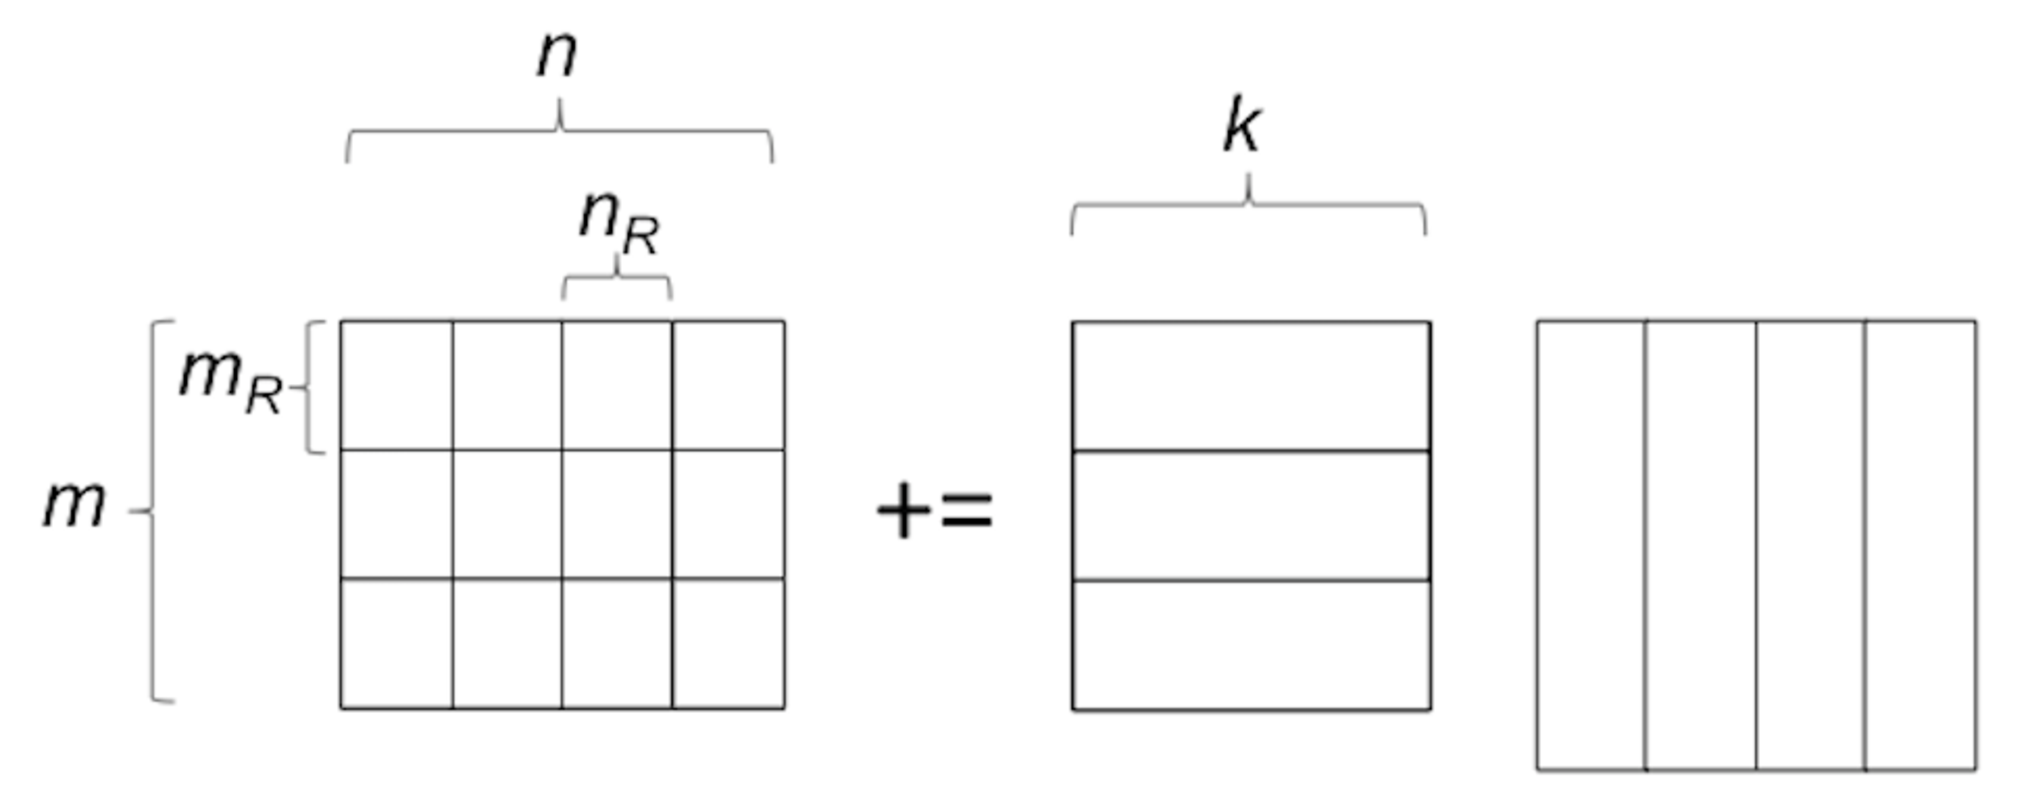
\includegraphics[width=3in]{figures/Step2.pdf}
\end{center}
What we want you to do is to write your code so that $ m_R \times n_R $ blocks of $ C $ are kept in registers.  
You get to choose $ m_R $ and $ n_R $, but you will want to update file {\tt include/bl\_config.h} with those choices.
This ensures that the test driver only tries problem sizes that are multiples of these block sizes, so you don't have to worry about ``fringe''.

\subsubsection{Vector intrinsics}

You will notice that even for smallish matrices, your implementation performs (much) worse than the implementations that are part of MKL and/or BLIS.  
The reason is that the compiler is not using the fastest instructions for floating point arithmetic.  These can be accessed either by using {\em vector intrinsic functions}, which allows you to explicitly utilize them from C, or by coding in assemply code.  For now, let's not yet go there.  We will talk more about this in Step 3.

